\section{Bus Interface}

Let us start with the most notable change we introduced to the \lib{libusbhost}
library. Yet before we do, we would like to describe the previous way how
\lib{libusbhost} supported USB HC drivers.

\subsection{Former State}

The library support was mediated by a single structure,
\struct{ddf_hc_driver_t}. This structure contained callbacks implementing
routines to initialize internal structures, start the HC, handle interrupt and
so on. Once the driver's DDF callback \fnc{dev_add} was called, the driver
passed the call to the library along with the \struct{ddf_hc_driver_t}
instance, which described how the HC is to be initialized. In one of the
callbacks, the driver called a function \fnc{hcd_set_implementation}, by which
it configured runtime operations.

From the perspective of data structures, the \lib{libubshost} defined
a structure for an instance of host controller, \struct{hcd_t}, and for
endpoint, \struct{endpoint_t}. Both structures had a field for storing driver
private data. The library also managed a device tree, with the device
structures stored inside DDF function nodes. The device structures were however
private for the library, and apart from two callbacks \fnc{ep_add_hook} and
\fnc{ep_remove_hook} the driver had no information about the devices. Also,
every endpoint could have two callbacks assigned by the driver, which were
called to alter maintenance of the Toggle bit (\fnc{toggle_get/set}).

The main work to be done by the driver is transfer management. For this
purpose, the library defined a structure \struct{usb_transfer_batch_t}, which
was created for every transfer and then passed to the driver's \fnc{schedule}
operation. The batch carried all the information about a USB transfer: target
address, pointer to the data buffer and its size, direction of the transfer and
so on. Along with this data, it carried one of two callbacks (in/out) to be
called after the transfer is finished. This particular callback was set by the
library, depending on the context from which a transfer was scheduled. Transfer
could be initiated either by the HC itself (e.g. reading the device descriptors
to determine match IDs for the DDF), or by the driver of the device via the IPC
interface methods (\fnc{usb_read} or \fnc{usb_write}).

In the first case, the driver called \fnc{hcd_send_batch_sync}, which created
a simple structure with completion flag, and the callback was set to a function
which filled the structure and toggled the completion flag. Then the issuing
fibril polled the completion flag until the transfer was completed. In a case
of a bus transaction issued by the device driver, the callback answered the IPC
call. The asynchronicity of HelenOS IPC fits this scheme perfectly.

Sometimes, if the request modified the internal state of the device (e.g. USB
ResetEndpoint request), the callback was wrapped in another callback, which
reset the endpoint's toggle after completion, and called the original callback.

The overall architecture of using callbacks passed as function arguments and
stored all around was really flexible, but very hard to read and understand.
Instead of simply tracing function calls, we needed to carefully study the
lifetime of the structure to track origins and modifications of these
callbacks.

Also, we felt that keeping driver-private data in a void pointer (with the
burden of maintaining the allocated memory) doesn't fit well for a library of
such a specific purpose. Instead, we decided to start a little revolution here.

\subsection{Current State}

The most notable change we introduced is a clear separation of the callbacks,
forming the interface of the HC driver against the \lib{libusbhost} library,
named the ``Bus interface'' in the figure \ref{fig:stack-architecture}. All the
runtime callbacks the library calls are contained in a single structure,
\struct{bus_ops_t}, which is defined by the driver. It is possible (and
recommended) that the instance of this structure is \mintinline{c}{static
const}, and a pointer to it is shared between all HC's the driver controls. The
names of the callbacks are ``namespaced'' by their first word, to clearly
distinct which entity the operation works with (\fnc{device_enumerate},
\fnc{endpoint_register}, \fnc{batch_schedule}, \dots).

Moreover, we defined a bunch of structures the library shares with the driver.
All of them use pointers and arrays to build a tree of entities the driver
works with. The lifetime of all entities is managed by the library, but the
driver is (with some exceptions) responsible for their allocation and
destruction. That gives the driver great flexibility in where the memory for
the structures will be allocated, and also how large the memory is. None of
them contains a void pointer to store private data, as its not necessary -- the
driver is supposed to allocate memory for a bigger structure if it needs it.

The C standard defines that pointer to a structure is equivalent to a pointer
to its first field. This promise is heavily relied on to implement
``inheritance'' of a C structures. To give an example, suppose that the driver
needs to keep more data about an endpoint. It then creates a structure for it:

\begin{code}
	typedef struct hc_endpoint {
		endpoint_t base;

		bool some_flag;
		unsigned more_data;
	} hc_endpoint_t;
\end{code}

Then, in the \fnc{endpoint_create} bus operation, it is supposed to create the
\struct{endpoint_t} structure. It allocates a space for \struct{hc_endpoint_t}
instead, and returns the pointer to its base field (which we know is the same,
but of different type). Whenever it then receives an \struct{endpoint_t *}
argument to a bus operation, it knows it is safe to typecast the pointer to
\struct{hc_endpoint_t *}, and work with the extended structure containing more
data.

All structures and their relations can be seen on figure
\ref{fig:hcd-memory-structures}. You can see that all of them have pointers to
their parent entities. That allows us to reduce number of arguments passed to
the bus operations, while retaining the flexibility needed to implement the
operations in different drivers. Lets walk through the entities one by one.

\begin{figure}
	\centering
	\label{fig:hcd-memory-structures}
	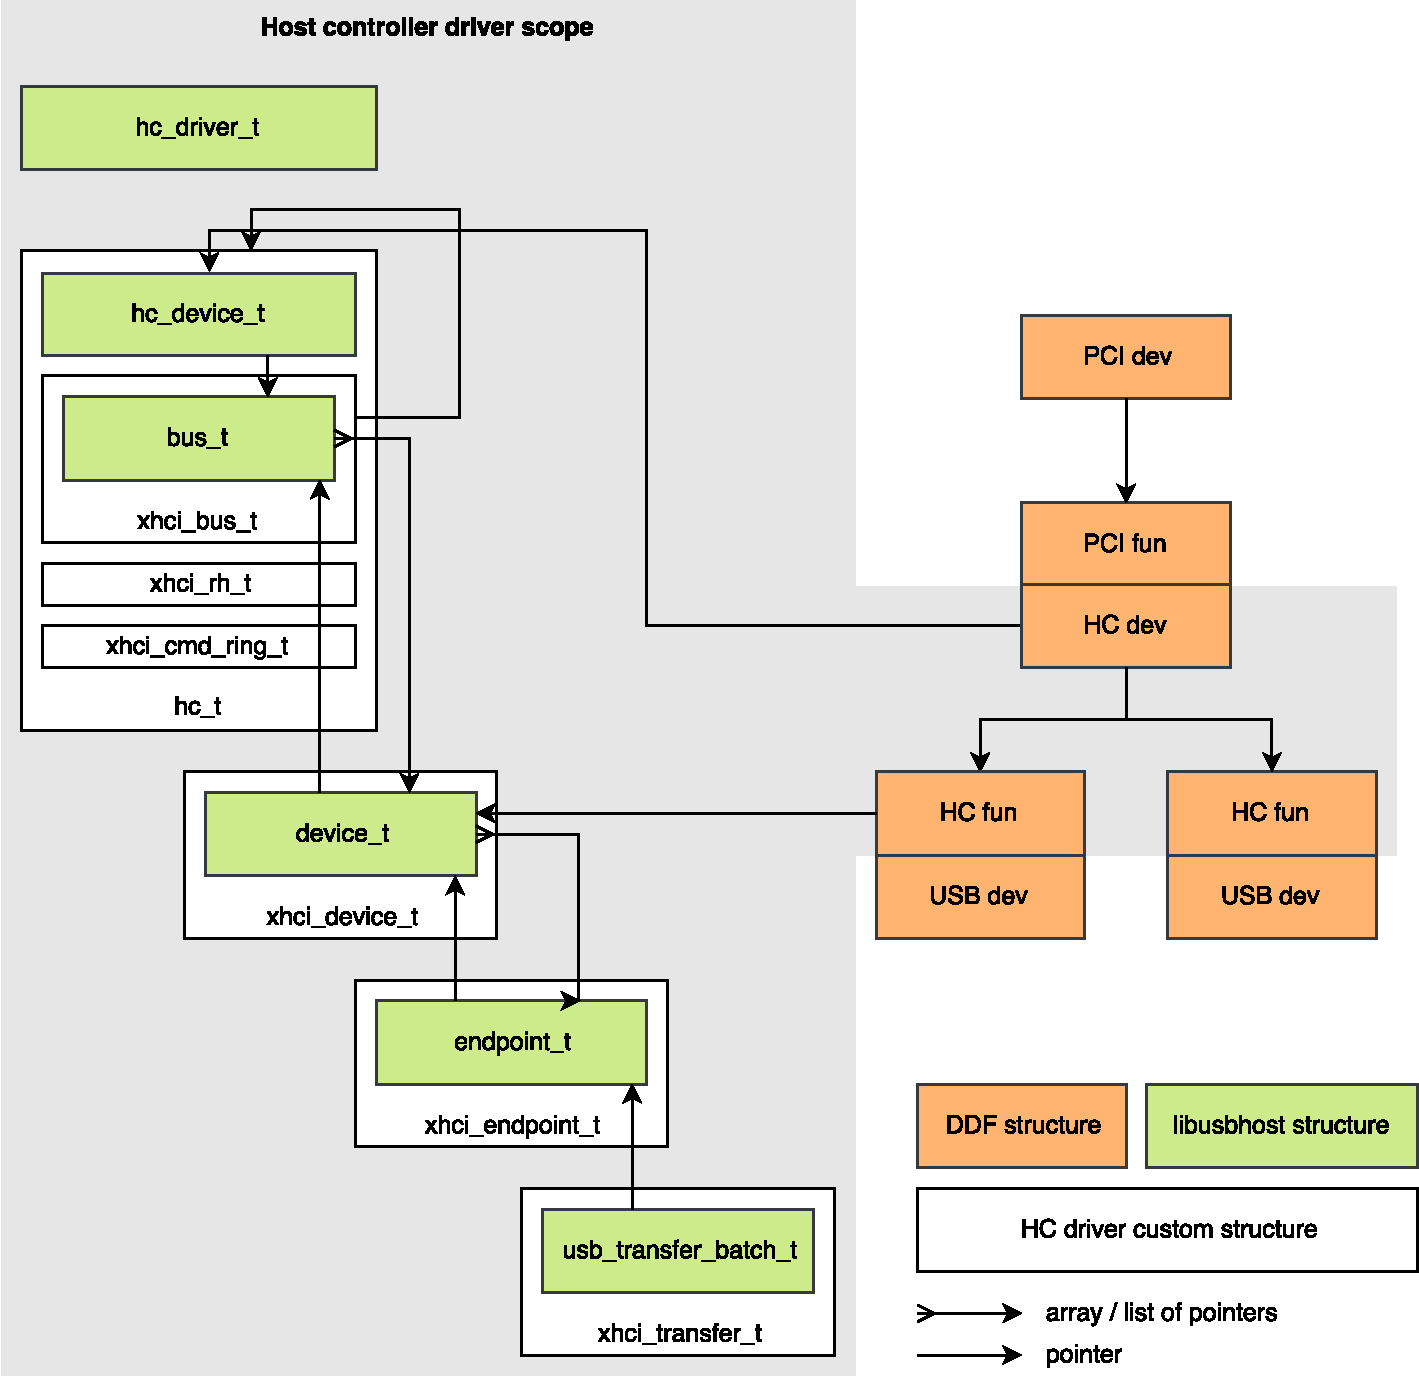
\includegraphics[width=0.5\textwidth]{hcd-memory-structures}
	\caption{Bus structures demonstrated on the example of how xHCI driver uses them.}
\end{figure}

\subsubsection{Structures Shared With the Driver}

\begin{description}
	\item[\struct{hc_driver_t}]
		Represents the driver instance. Created at the task startup (usually as
		a static instance), passed to the \fnc{hc_driver_main}. Contains
		operations to initialize a HC device.
	\item[\struct{hc_device_t}]
		Created by the library for every HC controlled. Contains pointers to
		the DDF device, control function, interrupt-replacement fibril. Shall
		be treated as opaque by the driver.
	\item[\struct{bus_t}]
		Created by the driver for every HC it controls. Manages the reservation
		of default address, keeps the pointer to bus operations. Strictly
		speaking, \struct{hc_device_t} and \struct{bus_t} represent the same
		entity -- the HC instance. They are separated to isolate responsibilities.
	\item[\struct{device_t}]
		Allocated inside the DDF function node for every USB device managed by
		the bus. Contains an array of endpoints registered for that device.
		Also, it contains a list of children \struct{device_t} structures, in
		case this device represents a hub. Because the topology presented to
		the DDF is flattened, this is the only place where the USB tree
		topology is stored.
	\item[\struct{endpoint_t}]
		Created dynamically at the time of registering an endpoint by the
		device driver. Contains information needed for scheduling and
		synchronization of scheduled transfers. Reference counted, as its
		lifetime can extend the lifetime of a device.
	\item[\struct{usb_transfer_batch_t}]
		Created dynamically at the time of initiating a transfer. Ownership
		travels across more entities, more information to be found in section
		\ref{sec:aborting-transfers}.
\end{description}

Now that we know the entities, we can introduce the operations expected to be
implemented by the HC driver.

\subsubsection{Bus Operations}

\begin{description}
	\item[\fnc{interrupt}]
		Process a hardware IRQ. Is passed a bus instance and a 32-bit status
		retrieved from the top half.
	\item[\fnc{status}]
		When the library fails to enable the IRQ, it starts a polling fibril
		instead. The polling fibril calls the status method to retrieve the
		status to be fed to the IRQ handler.

	\item[\fnc{device_enumerate}]
		When a (root)hub finds a new device, the library creates the DDF
		function node, and allocates a \struct{device_t} structure. This
		operation is then called to address the device and create the DDF match
		ids for it.
	\item[\fnc{device_gone}]
		Called when the hub signalizes a device is gone. Not required.
	\item[\fnc{device_offline} and \fnc{device_online}]
		The library calls these when the user requested the device to be brought
		offline/online. More information about this mechanism is in section
		\ref{sec:offline-online}.

	\item[\fnc{endpoint_create}]
		Called when the library needs to materialize an endpoint from the
		endpoint descriptor fetched from the device.
	\item[\fnc{endpoint_register}]
		When the device driver maps an endpoint descriptor, a pipe is created.
		On the HC side, respective endpoint is registered. The registration
		is performed by the library itself, this is just to let the driver do
		the HC-specific work.
	\item[\fnc{endpoint_unregister}]
		When the pipe is closed, the endpoint is unregistered. The HC is
		supposed to terminate all transfers on that endpoint before it returns
		from this operation.
	\item[\fnc{endpoint_destroy}]
		A function to free an endpoint and all allocated information. Called
		once the reference count drops to zero. If not specified, the structure
		is freed by \fnc{free}.

	\item[\fnc{batch_create}]
		Called by the library when a transfer needs to be initiated. If not
		specified, the batch is allocated by \fnc{calloc}.
	\item[\fnc{batch_schedule}]
		Called once the batch is ready to be scheduled.
	\item[\fnc{batch_destroy}]
		Once the batch is finalized and its completion callback is called, this
		function is supposed to free the memory. If not specified, the batch is freed by \fnc{free}.
\end{description}

Some operations do have generic implementation, so that the driver is not
required to implement them, a common behavior is implied. Others are required
only to support a specific functionality -- if not implemented, the
functionality is unavailable. Of course, functionality like the batch
scheduling is optional, but without it the driver is kind of useless.

The only callback that remains separated from the bus is the batch completion
callback. In order to support both synchronous batches from HC itself and
asynchronous batches from IPC, there needs to be a distinction. However, the
callback is no longer abused to implement additional functionality when the
transfer is finished.

To avoid duplicating functionality that was previously in the library and now is
supposed to be implemented by the driver, we created a module
\header|<usb/host/usb2_bus.h>|, which contains an implementation of some
operations relevant for USB2 and below. It implements address allocation, as
only xHC assigns addresses in hardware, older HCs leaves this responsibility on
software. The same holds for bandwidth management, which is further moved to
a separate module \header|<usb/host/bandwidth.h>|.

\subsubsection{Development of the Bus Interface Throughout the Project}

At first revisions, the bus interface was a bit richer. Also, it contained more
of the USB2 specifics hardwired -- like the bandwidth management. The impulse
to create the bus interface was the lack of systematic approach in the previous
solution, so it was a bit hard to understand. So we first did a refactoring
process, which moved all callbacks to the bus. For a long time, there was
a kind of runtime virtual binding of functions -- the older HCs used
\struct{usb2_bus_t} as their bus implementation, and overrode some of its
functions. As time passed by, we were able to identify and isolate parts that
could be separated cleanly and reduce the bus interface to its current state.

The result is not that much different from the former state -- only extended by
a few device-related callbacks, as xHC needs to know about devices, former HCs
need not. But the fact we needed to do the refactoring just to understand what
is going on proves the fact this interface must have been cleaned up and
defined more clearly. Also, the sharing of structures reduced the amount of
bookkeeping needed to be done by the drivers. This claim is supported by the
fact that even though we implemented new features and made performance
optimizations, the codebase of former HC drivers shrunk a few kilobytes.
